%=========================================================================
% (c) Michal Bidlo, Bohuslav Křena, 2008

\chapter{Úvod}
Tvorbou počítačových her se zabývá celé odvětví průmyslu, pracují na nich mnoha členné vývojářské týmy, i tak se vyvíjí měsíce i roky. Ale co vše se musí vlastně vytvořit, abychom se mohli projít ve virtuální 3D scéně? Tato práce popisuje implementaci jednoduché hry, dema, ovšem veškerá implementace bude směřována k případnému pozdějšímu rozšíření do plné hry. Vše bude řešeno buď vlastní implementací nebo \emph{freeware/open-source} knihovnami.
Práce se bude zabývat realizací základního osvětlení, načtení a vykreslení modelů, interakcí s uživatelem, dále vyřešením kolizí pomocí externí knihovny. K těmto cílům budou použity knihovny založené na \emph{OpenGL}, jmenovitě \emph{Assimp}\cite{assimp} pro načítání, \emph{Bullet physic engine}\cite{bullet} pro zachytávání kolizí a fyzikální model a \emph{irrKlang}\cite{irrklang} pro ozvučení a knihovny \emph{glew\cite{glew}, glfw\cite{glfw}, glm\cite{glm}} pro základní práci s grafikou.           

\chapter{Teorie}
V této kapitole bude popsána netriviální teorie později použita v aplikaci. Zaměří se primálně na teorii mnou implementovanou, nikoliv na teorii obslouženou knihovnami třetích stran. Jako hlavní zdroj pro tuto kapitolu slouží kniha Moderní počítačová grafika\cite{MPGbook}. 
\section{Phogův osvětlovací model}
Phongů osvětlovací model předpokládá, že většina světla nedopadá do kamery přímo, ale odrazem od objektů.
Toto odražené světlo dělí na tři složky \emph{Ambientní}, \emph{Difuzní} a \emph{spekulární}. Kdy Ambietní složka představuje světlo rovnoměrně rozptýlené v prostoru, tedy osvětluje všechny fragmenty stejně. Difuzní složka představuje světlo přímo od zdroje dopadající na fragment. Intenzita osvětlení difuzní složkou se odvíjí od úhlu dopadu, čím blíže k normále tím je fragment více osvětlen. Poslední složka, spekulární neboli zracodlová představuje světlo odrážející od fragmentu, tedy její viditelnost se mění na základě polohy kamery tzn. jak moc se světlo odráží směrem ke kameře. Phongův model v tomto případě předpokládá ideální odraz, tedy úhel dopadu se rovná  úhlu odrazu. Intezitu celkového ovětlení fragmentu můžem obecně spočítat vzorcem:
\begin{equation}\label{phong}
I_V = I_A r_a + \sum_{k=1}^{M}I_{L_k}[r_s(\vec{v}\cdot\vec{r_k})^h + r_d(\vec{l_k}\cdot\vec{n})]\cite{MPGBook}
\end{equation}
Vzorec \ref{phong} je obecný pro \emph{M} zdrojů světla. Já v aplikaci použiji jako zdroj světla jen slunce, takže můžeme vzorec zjednodušit na:
\begin{equation}\label{MyPhong}
I_V = I_A r_a + r_s(\vec{v}\cdot\vec{r_k})^h + r_d(\vec{l_k}\cdot\vec{n})
\end{equation}
 V obou vzorcích $ I_A $ je intenzita \emph{ambientní} složky a $r_a$ její barva. V první vzorci se pak sčítají všechny \emph{difuzní} a \emph{spekulární} složky všech zdrojů světla. V případě této práce se suma redukuje jen na jeden vzorek.

\section{Shadow depth map //TODO}\label{shadowMap}
\emph{Shadow depth map}, česky stínová paměť hloubky\cite{MPGBook}, je algoritmus na výpočet vlastních i vržených stínů hmotných těles. Vyznačuje se vysokou rychlostí výpočtu a nízkou kvalitou stínů, vyšší paměťovou náročností pro více zdrojů světla. Algoritmus spočívá ve vytvoření hloubkové mapy, podobně jako při řešení viditelnosti pomocí z-buffer algoritmu, kdy je v mapě uložená vzdálenost nejbližšího bodu ke zdroji světla. Při vykreslování se porovná hloubka daného bodu s hodnotou v mapě, pokud je vyšší není ve stínu jinak je. V důsledků použití rastrové mapy se u toho algoritmu projevují všechny problémy spojené s mapováním textur, jako aliasing, nízké rozlišení mapy. Dále může v důsledku nepřesnosti rasterizace vzniknout jemná odchylka a potom hloubka bodu vyjde o něco větší než při zápisu do hloubkové mapy a začne vrhat stín sám na sebe. Algoritmus této metody se dá zapsat jako:  
%\fbox{\parbox{\textwidth}{The \textit{two-step} model of XMCD:
	\begin{myEnumerate}
		\item pro každý světelný zdroj:
		\begin{myEnumerate}
			\item vykresli scénu z pohledu zdroje;
			\item pro každý pixel:
			\begin{myEnumerate}
				\item nejnižší z-souřadnici  ulož do mapy, "místo barvy";
			\end{myEnumerate}
		\end{myEnumerate}
		\item vykresli scénu normálně:	
				\begin{myEnumerate}
					\item pro každý fragment:
					\begin{myEnumerate}
						\item vec3 sum = (0,0,0); výsledná osvětlenost
						\item pro každou Shadow mapu $M_i$:
						\begin{myEnumerate}
							\item L-coord = souřadnice fragmentu v soustavě daného světla;
							\item if( $M_i$.get(L-coord.xy)<z):
								\begin{myEnumerate}
									\item sum += 0.5 * světlo;	//lezi ve stinu
								\end{myEnumerate}
							\item else:
								\begin{myEnumerate}
									\item sum += světlo;	// je osvětlen			
								\end{myEnumerate}
						\end{myEnumerate}
						\item sum /= počet světelných zdrojů;12
					\end{myEnumerate}
				\end{myEnumerate}
		\end{myEnumerate}


%}}
\section{Skeleton animation}\label{SA}
Skeleton animation je metoda inspirovaná stavbou lidského těla, tedy pohyb kosti způsobuje pohyb celé části těla a když pohnu například setehení kostí pohne se mi o stejnou rotaci i holení, vřetení kost i kosti kotníku a chodidla. Základní \emph{Skeleton animation} využívá dvě vrstvi síť bodů jako kůži a stromovou strukturu kostí viz. obrázek \ref{skeletalAnimation}. Pro jednoznačný popis a vykreslení animace potřebujeme znát:
\begin{itemize}
	\begin{item}
		pro vrchol:
			\begin{itemize}			
			\item pozici, uv souřadnice, normálu
			\item seznam kostí, kterými je ovlivněn
			\item seznam vah, poměr ovlivnění, pro tyto kosti
		\end{itemize}
	\end{item}
	\begin{item}
	pro kost:
	\begin{itemize}
		\item transformační matici pro přechod ze soustavy kosti do soustavy bodů
	\end{itemize}

\end{item}
	\begin{item}
	pro uzel:
	\begin{itemize}
		\item transformační matici pro přechod ze soustavy tohoto uzlu do soustavy rodičovského uzlu pro každý klíčový snímek animace
	\end{itemize}
	
\end{item}
	
\end{itemize}  
\begin{figure}
\begin{center}

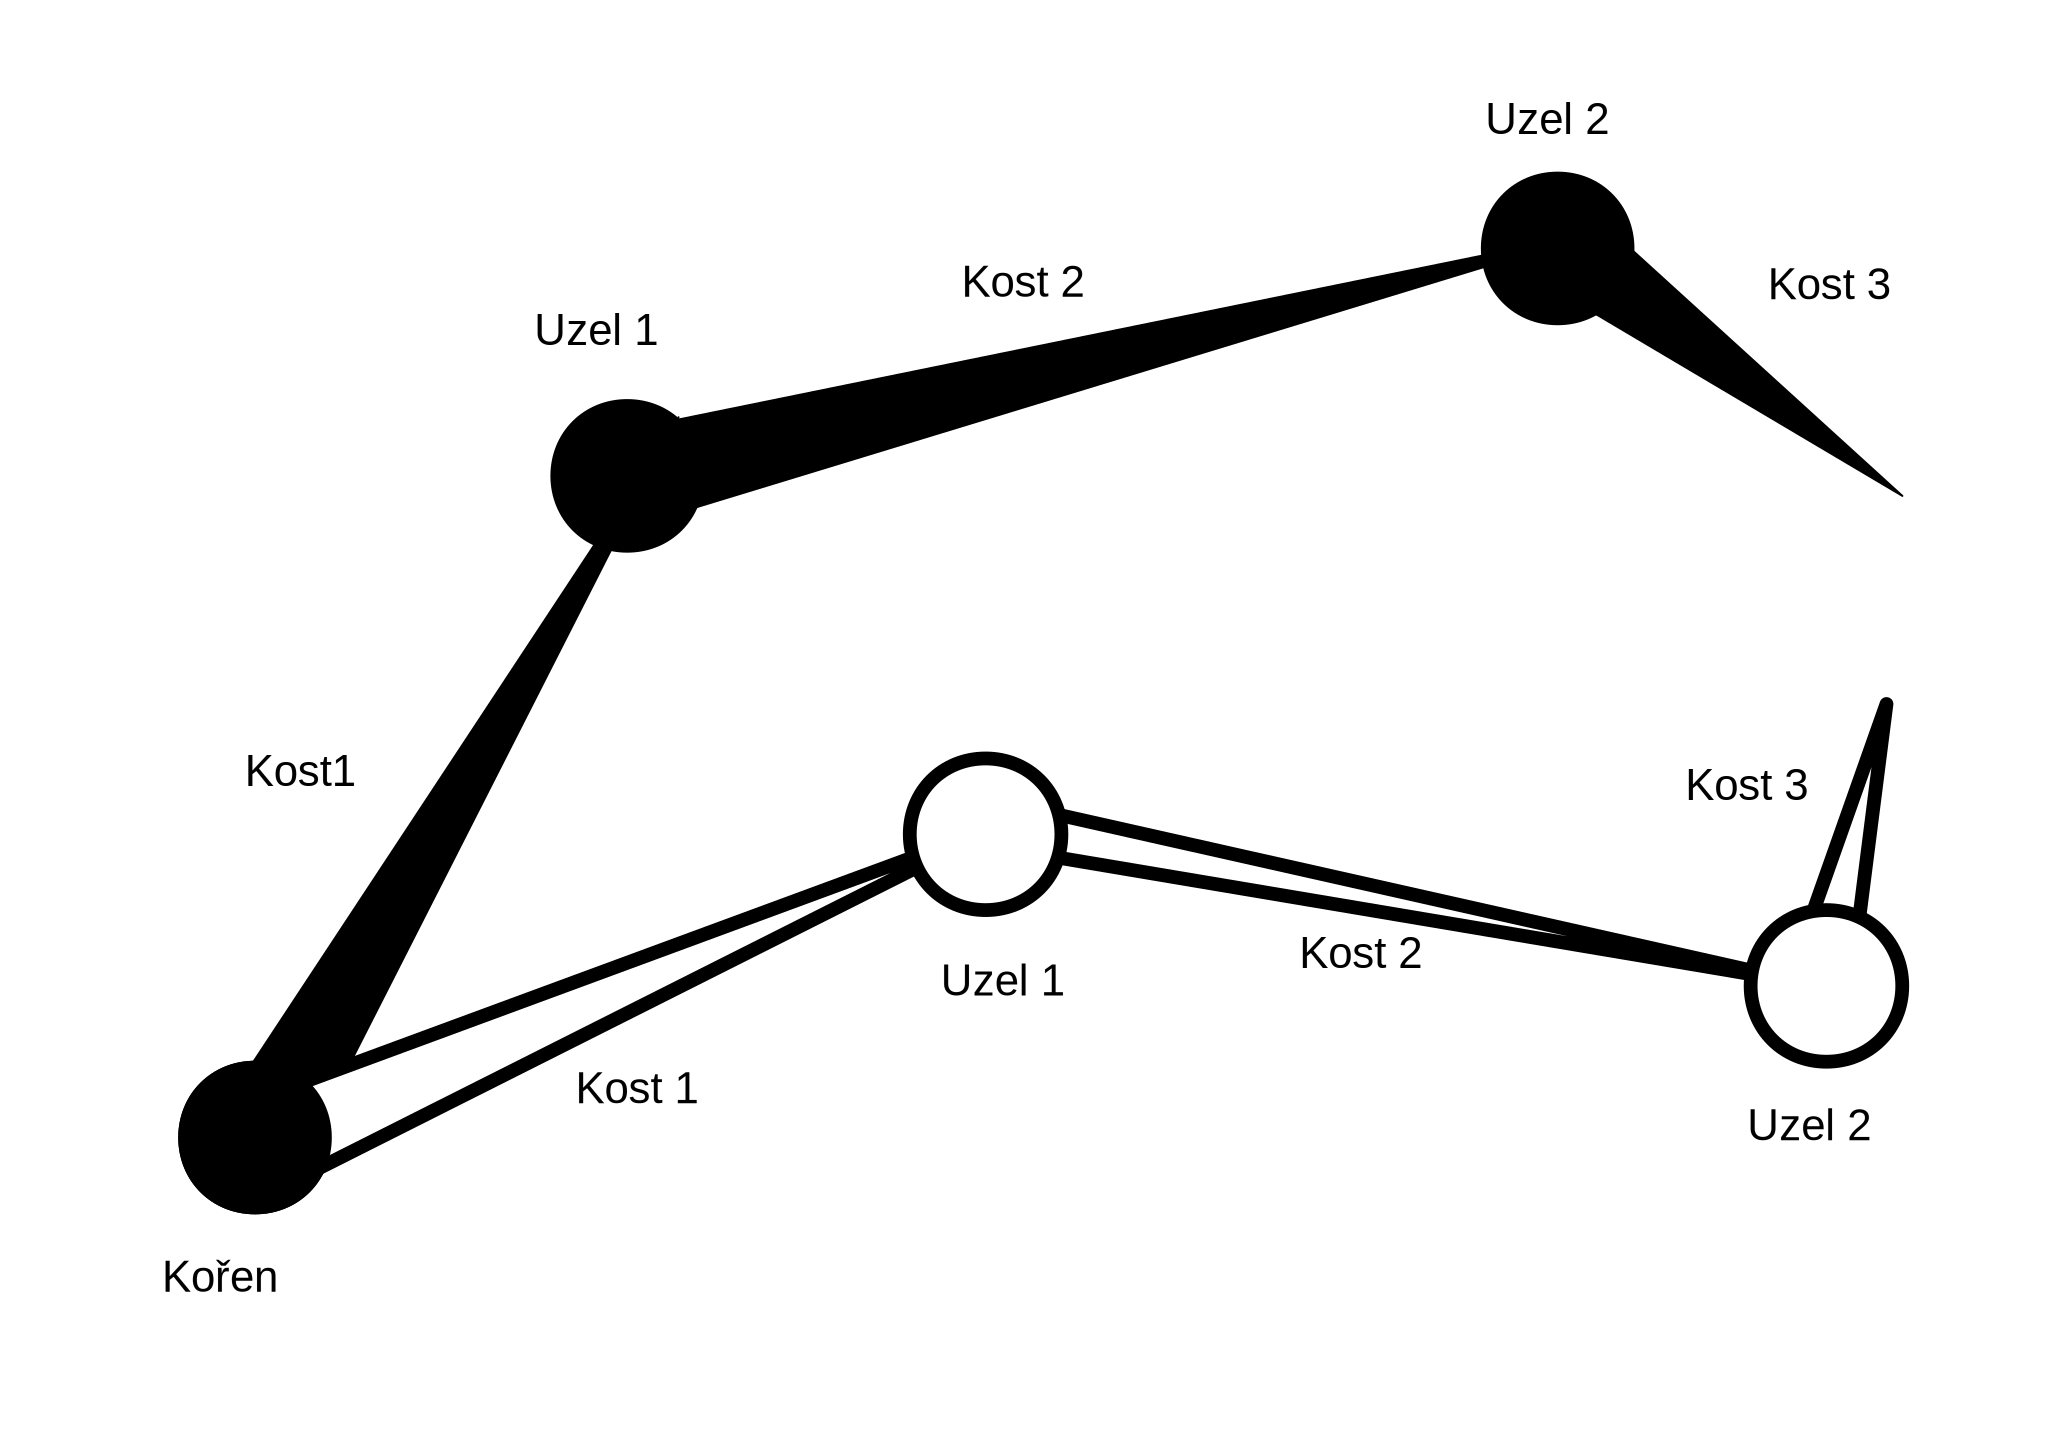
\includegraphics[scale=0.33 ]{obrazky-figures/skeletalAnimation}
\caption{Skelatal animation}\label{skeletalAnimation}
\end{center}\end{figure}
K výpočtu polohy vrcholu pro daný snímek se musí vypočítat kompletní transformační matice pro všechny kosti, kterými je vrchol ovlivněn. Každou z těchto matic se získá vynásobením všech matic uzlů od uzlu před danou kostí až ke kořeni násobeno ještě transformační matici kosti do soustavy bodů. Tyto matice po vynásobení příslušnými vahami a sečtení dají výslednou transformační matice pro daný vrchol. Stačí samozřejmě vypočítat pro každou kost matici jednou v daném snímku a pak ve vykreslování vrcholů k ní jenom přistoupit. Matice pro uzly se mění v závislosti na čase animace, ukládají se povětšinou jen matice pro klíčové snímky. Je-li čas animace mezi dvěma klíčovými snímky k určení matice pro každý uzel v čase t je třeba udělat vážený průměr matic z klíčového snímku před a po:
\begin{equation}\label{SAprumer}
M_t = \frac{M_{pred} * (t - T_{po})}{M_{po} *(T_{pred} - t)}
\end{equation}
Takže pro výpočet výsledné polohohy vrcholu bude vzorec bez optimaliazací(např. aby se každé kosti počítala jen jednou) bude vypadat takto:

\begin{equation}\label{SAvzorec}
M_t = \frac{M_{pred} * (t - T_{po})}{M_{po} *(T_{pred} - t)}
\end{equation}
  
\section{Perelinův šum //TODO}
\chapter{Návrh aplikace\label{Navrh_aplikace}}
První část této kapitoly bude pojednávat o obsahu a možnostech aplikace s důrazem na \emph{frontend}, tedy nebude se zabývat vnitřní implementací těchto možností. Druhá část pak následně probere použité způsoby pro realizaci těchto vlastností a zdůvodní proč tyto a ne jiné, případně se krátce zmíní o alternativách, zde budou take rozebráno použití knihoven třetích stran jako \emph{Assimp}\cite{assimp} nebo \emph{Bullet physic library}\cite{bullet}, dále jen \emph{Bullet}. Na závěr uvede diagram tříd a jeho popis. Podrobnosti k zajímavým částem implemntace těchto tříd a vlastností aplikace budou popsány v následující kapitole č.\ref{implementace} Implementace. 
\section{Obsah aplikace}
Cíle je vytvořit demo 3D hry, lukostřelecké střelnice. Demo bude tvořeno jen jednou scénou bez menu. Scéna bude obsahovat několik terčů a střeleckých pozic a umožňovat pohyb hráči v tomto prostoru, hráč bude vybaven  lukem a několika šípy. Dále hráč vždy uvidí \emph{head-up display}, dále jen \emph{hud}, složený z počítadla bodů, ukazatele síly a směru větru, ukazatele zbylých šípů a zaměřovače.Pro šípy bude zajištěno fyzikální chování a ovlivnění silou a směrem větru. Scénu osvětlíme pouze sluncem/měsícem dle herního času.
\subsection{Čeho všeho bude aplikace schopna}
\begin{itemize}
	\item Načítání a práce s modely a animacemi
	\item Fyzika letu a kolize objektů
	\item Osvětlení scény a stíny pro usnadnění odhadu vzdálenosti a realističnost
	\item Střídaní noci a dne
	\item Dostatečná náhrada slunce
	\item Vítr, plynulá změna jeho směru, poryvy, závětří
\end{itemize}
\section{Načítání, ukládání modelů a jejich animací}

Modelem se rozumí skupina vrcholů(angl. Mesh). Aby aplikace mohla model vykreslit musí být schopna jej načíst ze souboru a uložit si ho ve vhodné reprezentaci a vědět kterou texturu použít. K načtení bude použita knihovna \emph{Assimp}\cite{assimp}, aby bylo možné načítat více různých formátů. Ukládat se budou jako pole vrcholů, kdy vrchol bude představovat struktura obsahující pozici v souřadném systému modelu, uv koordináty, normálu a indexy a váhy kostí na které bude navázán, více v sekci \ref{SA} o \emph{skeletální animaci}. V tomto poli bude každý vrchol pouze jednou, neboť aplikace bude vykreslovat metodou \textbf{INDEX - zjisti odborný název}.
    
Animace jsou načítány společně s modelem ze souboru, \emph{Assimp} je ukládá do dynamického seznamu structur \emph{aiAnimation}. Každá z těchto struktur představuje jednu animaci modelu a vidět ji můžeme na obrázku\ref{aiAnimation}. 
\begin{figure}
	\begin{center}
		\includegraphics[scale=0.5]{obrazky-figures/aiAnimation}
		\caption{Část diagramu tříd knihovny \emph{Assimp}\cite{assimp}}\label{aiAnimation}
\end{center}\end{figure}

Vzhledem k tomu, že nad animací budou prováděny jen vyhledávací a čtecí operace je toto uspořádání dostačující. Pokud by ovšem vyhledávací a výpočetní funkce byly přidány do stejné třídy kde už jsou funkce pro práci s model, tak by se tato funkce stala velice přetíženou a těžko odladitelnou, vhodné bude zabalit tuto strukturu do vlastní třídy a obohatit ji o potřebné funkce a třídě model zpřístupnit jen výsledné transformační matice jednotlivých kostí.

 Modely se vyskytují ve spoustě různých formátech a variacích, rozhodl jsem se pracovat pouze se dvěma formáty:
\begin{itemize}
	\item \emph{Wavefront} od \emph{Wavefront Technologies} s příponou \emph{obj} pro modely bez animací
	\item \emph{COLLADA} od \emph{Sony Computer Entertainment} s příponou \emph{dae} pro modely s animacema.
\end{itemize}

Ke čtení modelů je sice použit \emph{Assimp::Importer}, který je schopen číst širokou škálu programů, ovšem aplikace je ozkoušena pouze na těchto dvou, při jiných formátech by potom mohlo dojít k problému při přiřazování do třídy \emph{Model} viz diagram tříd\ref{ClassDia}.
\section{Fyzika letu a kolize objektů //TODO}
Fyzikou rozumím výsledek působení sil ať už mnou vytvořených nebo vzniklých při kolizích objektů, zachytávání kolizí a tvorbu sil plynoucích z nárazu. Tuto stránku aplikace jsem se rozhodl vyřešit použitím knihovny třetí strany z důvodů relativně vysoké fyzikální složitosti a náročnosti na implementaci dostatečně rychlého algoritmu pro řešení kolizí. Zvolil jsem si knihovnu \emph{Bullet}, která poskytuje možnost řešit jak zachytávání kolizí, tak jednoduché zajištění fyzikálního chování pevných objektů i měkkých objektů Ovšem \emph{bullet} provádí výpočty na základě vlastní fyzikální scény, je tedy potřeba zajisti provázání mezi fyzickou reprezentací modelu a jeho entitou určenou pro vykreslování. Vazba musí být obou směrná neboť model se v každém vykreslovacím cyklu musí být schopen dotázat na polohu jeho fyzikálního ekvivalentu, a opačně, protože \emph{Bullet} vrací kolize v jako pole dvojic \emph{btColisionObject} a pro tyto objekty se musí zavolat příslušná funkce(výpočet bodů za zásah, zafixování polohy vůči zasaženému tělesu, ...).      
\section{Osvětlení a stíny //to finish}
Scénu bude osvětlovat jen jedením až dvěma  zdroji směrového světla představující slunce a měsíc za použití Phongova osvětlovacího modelu. Jeho poloha a intenzita se bude měnit dle herní denní doby.   
Stíny budou vypočteny a vykresleny metodou \emph{shadow maping }jenž je popsána v kapitole \ref{shadowMap}. Protože aplikace bude mít jen jeden až dva směrové zdroje světla je tato metoda vhodná díky své rychlosti a tvoří se jen jedna - dvě mapy. Tato mapa se bude přepočítávat pro každý snímek může me ji tedy vždy namapovat tak, aby měla co nejmenší přesah přes plošné promítnutí tělesa vymezeného pohledem kamery a zdroje světla. Tento způsob namapování umožňuje pracovat s menší texturou, tím rychlejší výpočet a méně zabrané paměti. 
\section{Střídání noci a dne}
Na \emph{skybox} budou na mapovány celkem tři textury, pro mraky, denní a noční oblohu. Mraky budou vidět vždy, v ideálním případě se budou měnit pomocí \emph{Perlinova} šumu. Střídání noci a dne je způsobenou změnou poměru míchání noční a denní textury pro jednotlivé fragmenty.

    \begin{figure}
    	\begin{center}
    		\includegraphics[scale=0.35]{obrazky-figures/dayOnight}
    		\caption{Graf střídání denní a noční oblohy}\label{dayOnight}
    \end{center}\end{figure}

Poměr pro každý fragment je dán mezi úhlem jeho osou(polopřímka ze středu přes něj) a osami 1 a 0, jak je vidět na obrázku \ref{dayOnight}.Pokud se fragment nachází ve stejném kvadrantu jako osa 0 je poměr vypočítán na základě jeho úhlu, je-li úhel 45\degree  je poměr je 0:1 v neprospěch aktuálního cyklu naopak pro -45\degree  1:0 pro aktuální cyklus. Mezi těmito hodnotami je potom nepřímá úměra. Ve zbylých třech kvadrantech je poměr vždy buď 1:0 nebo 0:1, odvíjí se toho, která čtvrtina  denního/nočního cyklu je:
\begin{itemize}
	\item kvadrant u osy 1:
		\subitem pro 1 - 3 část cyklu 0:1
		\subitem pro 4 část cyklu 1:0 
	\item kvadrant naproti ose 0:
		\subitem pro 1 a 2 část cyklu 0:1
		\subitem pro 3 a 4 část cyklu 1:0 
	\item kvadrant naproti ose 1:
		\subitem pro 1 část cyklu 0:1
		\subitem pro 2 - 4 část cyklu 1:0 
\end{itemize}
Celý den má tedy 8 částí, 4 denní a 4 noční, trvá dvě otočení os o 360\degree. Aplikace při spuštění začíná v čase nula, což je úsvit nového dne. 
\section{Slunce a měsíc} 
Slunce a měsíc se realizují pomocí plochých modelů rotujících kole středu \emph{skyboxu}. Doba oběhu musí trvat celý den, tedy dvě otočení os \emph{skyboxu}. V rámci třídy pro Slunce a měsíc se bude řešit i změna směru světla příslušného objektu. Pro správný pohy se musí zajisti dvě věci správné natočení plochy objektu, aby nebyl vidět jako elipsa či jako pouhá čára, uchování vzdálenosti od středu \emph{skybox}, potažmo avatára. Dosáhne se toho pomocí vektoru $\vec{a}$ mezi středem a objektem a rotací $\vec{a}$ i objektu kolem stejné osy(vyjádřená stejným předpisem, počítána vždy v relativní soustavě objektu nebo globální soustavě v případě $\vec{a}$). Poloha objektu se potom vždy nastaví podle vektoru $\vec{a}$ posunutého do aktuálního středu \emph{skyboxu}.
\section{Vítr}
Vítr je na vykreslování relativně jednoduchý jev, není totiž vidět, ale na druhou stranu má spoustu viditelných projevů. Zatím se bude práce zabývat jen působením větru na šíp za letu.
Vítr bude mít globální sílu a směr, které se budou v čase měnit, změna bude vypočtena po každé herní vteřině pomocí perlinova šumu. Tak to by vznikl vítr, který by všude byl stejný, jenže vítr se mění, dá se zastavit a vznikají závětří, tady pofukuje víc, tady méně, tamhle trochu jiným směr a tak, aby se dalo dosáhnout tohoto chování aspoň do určité míry realističnosti musí se učit závětrná míst, větrné stíny, a pro každý bod vypočíst drobnou odchylku směru a síly jak je znázorněno v obrázku \ref{windmap}.

\begin{figure}
	\begin{center}
		\includegraphics[scale=0.5]{obrazky-figures/windMap}
		\caption{Větrná mapa výsledné aplikace}\label{windmap}
\end{center}\end{figure}
Na obrázku \ref{windmap} nám směr a velikost větru znázorňují šipky. Za oběma čtverci jsou vidět větrné stíny s výrazně nižší intezitou větru. K výpočtu větrných stínů se dá použít téměř jakákoliv osvětlovací metoda, proto že vítr se v podstatě ničím neliší od světla, stále jsou to paprsky/proudy, jen jejich projev je jiný místo osvětlení místa dopadu jej posunou. Já jsem se rozhodl použít metodu \emph{shadow maping} a znovu použít již nutně implementované funkce pro výpočet stínů osvětlení. Tímto postupem lze získat větrné stíny, ale jinak se síla a směr větru nijak nebude měnit. Proto výslednou mapu ze \emph{shadow mapingu} zašumíme, například již zmíněným \emph{perlinovým šumem}.Jsou dvě možnosti buď použít 2D perlinův šum na celou mapu nebo 1D pouze na aktuálně čtený bod. Vzhledem k tomu, že vítr bude ovlivňovat jen několik těles a pro každé těleso se bude vyčítat jen jeden bod z mapy,vysvětlím dále, bude rychlejší na výpočet použít pouze 1D šum při čtení.

Zbývá vyřešit jak se bude vítr projevovat, lze k tomu  přistoupit dvěma způsoby jednodušším a méně reálným nebo  složitým a reálným. Jednoduší znamená, vítr se projeví jako pouhá směrová síla, bez ohledu na dopadovou plochu na tělese. Složitý znamená, že vypočítat dopadovou plochu z ní odvodit výslednou sílu větru. K zjištění dopadové plochy bychom museli ovšem každý fragment tělesa otestovat kde leží v mapě, jestli je ve stínu nebo ne. Pokud se tento test prováděl na CPU, došlo by k výraznému zpomalení aplikace, na GPU by to nebyl problém a v ničem by se to nelišilo od vykreslování stínů, ovšem standardní knihovny pro práci s GPU neumožňují přesun dat z GPU zpět do CPU. Pokud by šlo o simulátor plachetnice tak by se určitě muselo jít složitější cestou, ovšem tím že v rámci práce tvořím lukostřeleckou střelnici a větrem budou primárně ovlivněny šípy, které mají malou plochu a v podstatě stejnou ze všech stran, bude dostačující jednoduchá cesta. Z toho i vyplívá proč se bude vždy číst jen jeden bod mapy pro těleso a stačí tím pádem 1D šum.   
\chapter{Implementace \label{implementace}// TODO}
\section{Diagram Tříd// TODO popis}
Na obrázku \ref{ClassDia} je zjednodušený diagram tříd výsledné aplikace. Aplikace je složena ze tří hlavních částí:
\begin{enumerate}
	\item Třída Scene, která zapouzdřuje celou aplikaci.
	\item Třída BulletWorld, přes kterou je řešena veškerá fyzika.
	\item Třída Model, která je výchozí třídou pro většinu prvků ve scéně.
\end{enumerate} 
Dále pak aplikace má mnoho dalších tříd, jako třídy pro HUD nebo pro práci s animacemi či zvukem, mezi zajímavější pak patří třídy \emph{Skybox} a \emph{SunMoon}, které mají na starosti celé střídání noci a dne a pohyb zdrojů světla. 
\subsection{Třída Scene}
Třída Scene je ústřední třídou, z ní se přistupuje do třídy BulletWorld pro detekci kolizí a změny poloh modelů na základě působení sil, zde se také řeší jednotlivé kroky vykreslování jako vykreslení do \emph{wind mapy, shadow mapy} a výsledné.

Třída tím pádem obsahuje převážně funkce pro nastavení objektů, jejich vkládání případné nastavení propojení mezi objekty, které spolu nějak komunikují(např.:zbraň a projektil nebo objekt a jeho fyzikální představitel). Většina chování objektů je v jejich vlastní režii, třída Scene volá jen funkce pro jejich nastavení při vzniku a během cyklu už jen vykreslovací funkce.  

Tato třída ještě obsahuje slovníky načtených modelů a textur. Slovník pro modely má tvar <cestaKsouboru,ImportModel>. Při načítání souboru se zkontroluje zdali již není ve slovníku, je-li použije se příslušný záznam, není-li tak se soubor načte a zpracuje do třídy ImportModel a vrátí se opět záznam ze slovníku. U textur to probíhá podobně jen místo třídy ImportModel se použije přímo adresa textury na GPU.
\subsection{Třída BulletWorld}
  
\begin{figure}
	\begin{center}
		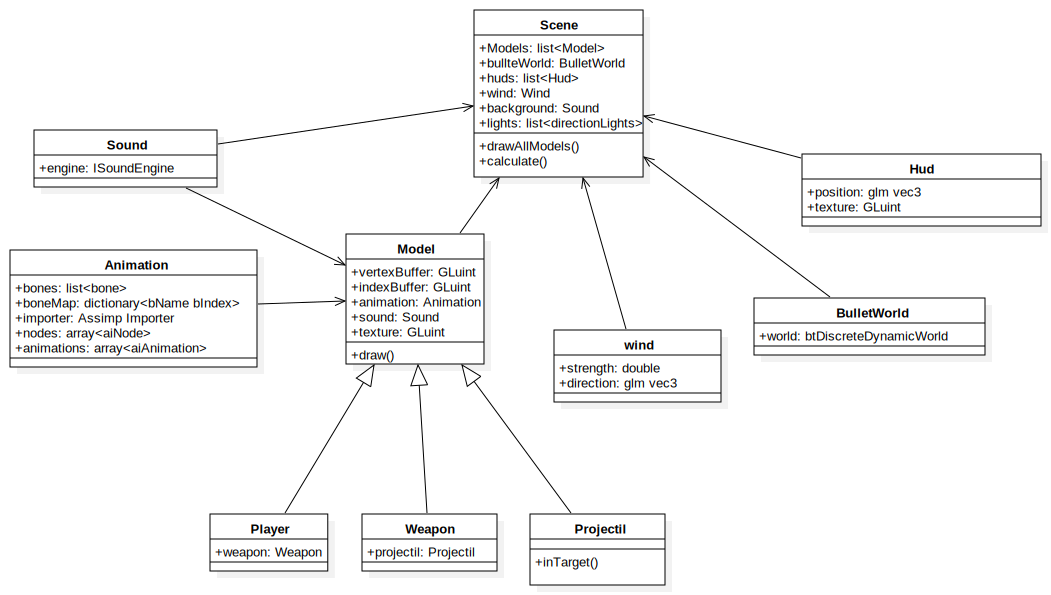
\includegraphics[scale=0.5]{obrazky-figures/ClassDia}
		\caption{Zjednodušený diagram tříd výsledné implementace}\label{ClassDia}
\end{center}\end{figure}


\section{Zajímavé nebo problémové části implementace}
	\begin{itemize}
	 	\item problémy při implementaci větru
	 	\begin{itemize}
	 		\item nekonečnost stínu
	 		\item simulace přirozených poryvů větru 
	 	
	 	\end{itemize}
	 	\item skeleton animation
	 \item zajištění jednoho načtení modelu		
	
	\end{itemize}

\chapter{Shodnocení náročnosti a efektivnosti implementace// TODO}
\begin{itemize}
	\item paměťová náročnost ku počtu modelů
	\item jak vylepši tuto věc
	\item framerate
	Obsah...
\end{itemize}
\chapter{Závěr// TODO}
%=========================================================================
